\section{Introduction}

\Xten{} is an experimental new language currently under development at
IBM in collaboration with academic partners. The \Xten{} effort is part of
the IBM PERCS project (Productive Easy-to-use Reliable Computer Systems)
in the DARPA program on High Productivity Computer Systems. The PERCS
project is focused on a hardware-software co-design methodology to
integrate advances in chip technology, architecture, operating systems,
compilers, programming language and programming tools to deliver new
adaptable, scalable systems that will provide an order-of-magnitude
improvement in development productivity for parallel applications. It is
expected that applications written in \Xten{} will execute over
high-performance interconnects using low-level communication libraries.
\Xtenlib{} is a library that is built on top of low level communication
libraries, like LAPI~\cite{LAPI} and provides a runtime target API for
the \Xten{} compiler.

\begin{figure}
\center
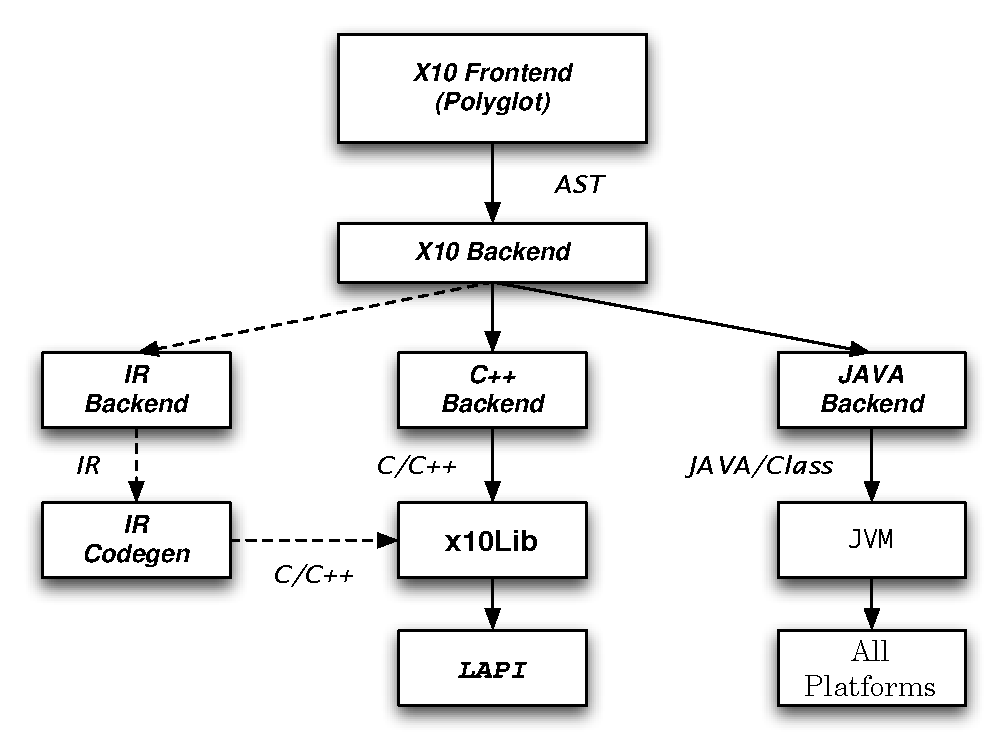
\includegraphics[scale=0.5]{figs/x10-block.pdf}
\caption{Overview of Implementation Strategies for \Xten{}}
\label{fig:x10-block}
\end{figure}

Figure~\ref{fig:x10-block} depicts the implementation strategy for the
\Xten{} programming language. The \Xten{} backend is responsible for
converting \Xten{} programs to map to either the C++ backend or the
{\sc{Java}} backend. The C++ backend then links with the \Xtenlib{} API
to run over high-performance interconnects on multiple places, i.e. on
multiple processes spread out over different nodes connected by a
network. The {\sc{Java}} backend is used to run \Xten{} programs in the
context of a JVM. In this document, we will focus only on \Xtenlib{}.
The Low-Level Communication API (LAPI)~\cite{LAPI} is utilized by
\Xtenlib{} to communicate over the network. This provides a highly
optimized runtime library.

The primary purpose of \Xtenlib{} is to provide the \textit{Partitioned
Global Address Space (PGAS)} required by \Xten{} along with methods to
deploy and execute \Xten{} programs. \Xtenlib{} provies the PGAS by
logically dividing up the address space among the various computing
processes and managing the book-keeping required to convert
pointer-dereferences into communication calls. \Xtenlib{} borrows the
process management framework from Parallel Operating Environment (POE),
which is ordinarily used to run MPI applications. Thus, inheriting a
highly optimized and scalable runtime environment.

The rest of this Section outlines the design goals and summarizes
desired functionality.

\subsection{Design Goals}
\Xtenlib{} is a runtime system for \Xten{}~\cite{x10}. 
We list the following explicit design goals for \Xtenlib:
\begin{itemize}
{}\item \Xtenlib{} should permit current C/C++ MPI programmers to
 program with \Xten{} concepts such as global shared memory,
 multi-threaded places, asyncs, futures, clocks and one-sided memory
 operations.

 {}\item \Xtenlib{} should export an interface to the compiler
 similar in spirit to the interface provided by the Java Virtual
 Machine. The interface must provide specialized entry points for
 common cases (e.g.{} allocating 1d, 2d, 3d rectangular arrays).

\item It should be possible to spawn activities in the current 
  process or on remote processes, and detect quiescence and
  termination of these activities.

{}\item The library should be available in C and C++ and usable within
MPI programs.

{}\item The library should be layered on top of a {\em Messaging API}.
  The Messaging API should be efficiently implementable on top of
  LAPI~\cite{lapi}, ARMCI~\cite{armci}, GASnet~\cite{gasnet} and other
  similar high-peformance messaging systems.

  {\em We may choose to build directly on top of GASNet.}

\item Data-structures should be designed for scalability.

\item The design should efficiently execute programs that are 
 communication-intensive and programs that are compute-intensive. It
 should permit the programmer to specify how many processes to run on
 each node of the cluster, how many places to run on each process, and
 how many threads to assign to each place.
\end{itemize}
Initially bindings will be provided for C and C++. Bindings for Fortran
and Java are also planned.

The following are explicitly {\em not} design goals for \Xtenlib:
\begin{itemize}
{}\item \Xtenlib{} is a C/C++ API: it will not offer any explicit
support for statically proving properties such as deadlock-freedom.
(Such properties are provided at the language level for \Xten).
{}\item This version of \Xtenlib{} will not provide any support for
garbage collection. The user is responsible for automatically managing
the lifetime of objects. (Functions will be provided to allocate space
in the global shared memory.) 

{}\item This version of \Xtenlib{} will not support the dynamic creation of places.

{}\item This version of \Xtenlib{} will not support checkpointing of
places. It will not support migration of places from one process to
another.

{}\item Distributed data strutures other than arrays will be provided in a subsequent release.

\end{itemize}

\subsection{Summary of desired functionality}
\Xtenlib{} provides functions to do the following:

\begin{itemize}
\item Get a remote (globally valid) reference for a local data structure.

  Such references can be passed from place to place and still remain
  valid. Two such references may be checked locally (without any
  communication) to determine if they point to the same data
  structure.

\item Spawn an async at a specified place, with a given function pointer
  and arguments, and clocked on given clock set. (The place may be
  specified either through a specific structure naming the place or
  through a remote reference.)

%  The X10 model does not require that an async intended to be executed
%  at the current place (or another place in the current area) is in
%  fact executed by a different thread. It only requires that X10
%  progress guarantees be preserved. In particular, it is legal for an
%  X10 implementation to execute an async inline (and/or use a more
%  sophisticated work-stealing algorithm) if the async does not invoke
%  any externally blocking operation (e.g. a next operation on an old
%  clock, or a conditional atomic operation).

\item Create a clock, and perform clock operations (next, resume, drop).

\item Spawn a future at a given place, with a given function
  pointer and arguments, and clocked on given clock set, and return
  the future.

\item Force the future. (This causes the current thread to block until the
  future value has been computed, and must therefore be performed at
  the top-level.)

\item Spawn activities in parallel at a given vector of places.

\item Terminate the current activity. (This does not terminate the current
  pthread, merely causes it to look for another activity to execute.)

\item Call finish to suspend on the termination of all asynchronous
  activities in the scope of the finish.

\item Perform an atomic operation with a given piece of code.
\item Throw an exception (to be caught by an enclosing finish).

\item Initialize a global data structure by allocating local arrays at
  given places.

{}\item Perform operations on the local portion of an array --
read/write/atomically update/iterate over elements in storage
order/region order.

{}\item Copy a portion of an array from the local place to a remote
place, or from a remote place into the local place.

{}\item Perform reduction operations on a global array.

\item Free global or local data structure.
\end{itemize}

Additional intrinsics capturing common idioms for communication that
can be efficiently executed on modern hardware will also be provided.

\paragraph{Target architecture}
The intended target architecture for the initial \Xtenlib{}
implementation is a cluster of SMPs connected through a high
performance switch. For instance, a cluster of 64-way Power5 SMPs
connected by a Federation switch. We view this as the best current
approximation to the PERCS machine being designed for 2010. We expect
the current design to be applicable to the PERCS machine though the
details may change significantly.

%\subsection{Design questions}
%
%Will the design exploit intra-place parallelism?
%
%Global arrays are allocated relatively infrequently. (But many
%activities in multiple places may simultaneously allocate multiple
%global arrays.)
%
%\subsection{Design point}
%One thread per place. We will 

\subsection{Overview of the design}
An \Xten{} {\em job} consists of a number of \Xten{} operating system
{\em processes}, each running on an SMP. (A single SMP may host
several processes in the same job.) Each process {\em hosts} one
place, and uses one or more application-level threads to execute
the asyncs in these places. Each process uses the messaging layer to
communicate with other processes. On being launched a job consults
some configuration information to determine how many processes are to
be started at different nodes in the cluster.  On being launched each
process initializes its internal data structures, and synchronizes
with all other processes to coordinate its initial state.

Each process maintains a collection of threads and a (double-ended)
queue of asyncs per place. The threads associated with a place suspend
waiting for a new activity to be added to its queue. This activity may
be added as a result of the execution of an async at a different place
in the current process, or on receipt of an ``active message'' from
the messaging layer.

When a thread is awakened it pulls the next async out of the queue,
determines whether the blocking condition (if any) associated with the
activity is satisfied and then executes it to completion. If the
condition is not satisfied then object corresponding to the async is
suspended on the condition variable. It will be awakened (and added
again to the activity pool) once there is reason to believe its
condition has changed.

An async is represented as an object with a particular interface.
Asyncs are classified statically based on the characteristics of the
code they run: {\em nonblocking} (code does not perform a conditional
wait on some variable), {\em local} (executing in the same place),
{\em immediate} (can be executed without acquiring a lock). Blocking
asyncs are required to be {\em top level} blocking: the call to
conditional wait must not occur within a method call. During execution
an activity $A$ may spawn new asyncs. If the new async is to be
executed at a different place in the current node and is immediate, it
may be performed immediately by the thread executing $A$.  If the new
async is local and nonblocking (or immediate) it will be executed
immediately (by the spawning activity).  For all other asyncs intended
to execute at another place in the same process, an object is created
and added to its queue of asyncs. If the new async is intended to
execute at a remote place then a LAPI active message is queued for the
target place. 

The compiler may use static analysis and type information to
determine that an activity should be inlined (e.g.{} because it is
local and immediate). Such activities do not even show up as
activities in the runtime system. In particular the compiler is
strongly encouraged to examine the bodies of asyncs and determine if
they can be classified as immediate/local/nonblocking.

An async may be associated with some synchronization-related
data-structures, such as the clocks on which it is registered.
%\paragraph{Implementation of Global Address  Space}

\paragraph{Implementation of atomic operations}
{}\Xtenlib{} provides special kind of objects, {\em monitored} objects
(e.g.{} futures). Each monitored object is a normal \Xten{} object
together with a data-structure (the suspension queue) for recording
the activities that are suspended on this datum, waiting for it to
change state. Writes to fields of monitored objects result in the
suspension queue being examined. The suspension predicate for each
async in the queue is evaluated, if it is true the async is moved from
the suspension queue to the async queue associated with the place.
